\documentclass[12pt,ignorenonframetext,dvipdfmx,cjk,hyperref={bookmarks=false,compress,slidestop}]{beamer}
\usetheme{GrayGradient}
\usepackage[T1]{fontenc}
\usepackage[utf8]{inputenc}
\usepackage{amssymb,amsmath}
\usepackage{lmodern}
\setcounter{secnumdepth}{0}
\AtBeginDvi{\special{pdf:tounicode EUC-UCS2}}
\renewcommand{\kanjifamilydefault}{\mgdefault}
\renewcommand{\baselinestretch}{1.4}
\usefonttheme{professionalfonts}
\usepackage[sc]{mathpazo}
\usepackage[scaled]{helvet}
\usepackage[scaled]{beramono}
\usepackage[deluxe,expert]{otf}
\usepackage{textcomp,okumacro}
\usepackage{url}

\title{プレゼン}
\author{金子達哉 \texttt{(id:catatsuy)}}

\begin{document}
\frame{\titlepage}

\begin{frame}\frametitle{自己紹介}

\begin{itemize}
\itemsep1pt\parskip0pt\parsep0pt
\item
  金子達哉
\item
  はてな ID: catatsuy
\item
  twitter: catatsuy
\end{itemize}

\begin{picture}(0,0)(0,0)
  \put(200,0){
\includegraphics[clip, height=35truemm]{catatsuy}}
\end{picture}

\vspace{-20pt}

URL:

\begin{itemize}
\itemsep1pt\parskip0pt\parsep0pt
\item
  \url{http://www.catatsuy.org}
\item
  \url{http://blog.catatsuy.org}
\item
  \url{https://matw.co}
\end{itemize}

\end{frame}

\begin{frame}\frametitle{所属}

\begin{itemize}
\itemsep1pt\parskip0pt\parsep0pt
\item
  東京工業大学
\item
  情報工学科 4 年(9 月卒業予定)
\item
  吉瀬研究室

  \begin{itemize}
  \itemsep1pt\parskip0pt\parsep0pt
  \item
    コンピュータアーキテクチャ
  \end{itemize}
\end{itemize}

\end{frame}

\begin{frame}\frametitle{就職活動}

\begin{itemize}
\itemsep1pt\parskip0pt\parsep0pt
\item
  はてなインターン 2012
\item
  pixiv インターン
\end{itemize}

\vspace{-20pt}

\begin{center}
 \begin{tabular}{cc}
   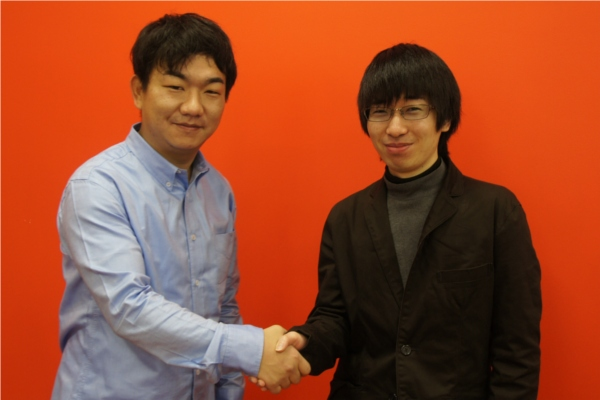
\includegraphics[clip, height=38truemm]{pixiv} & 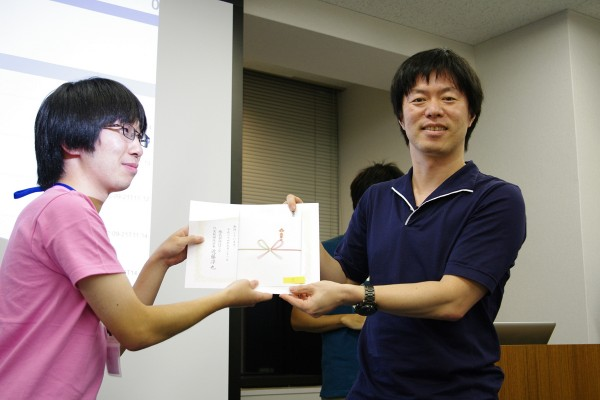
\includegraphics[clip, height=38truemm]{hatena} \\ 
  \end{tabular}
 \end{center}

\end{frame}

\begin{frame}[fragile]\frametitle{verb 環境}

\begin{verbatim}
#include <stdio.h>
int main() {
  printf("hello, world\n");
  return 0;
}
\end{verbatim}

\end{frame}

\end{document}
